\section{Concurrent Programming}

There is sometimes a conflation between concurrency and parallelism, two related but different methodologies. \emph{Concurrency} describes actions/computations that occur at the same time, whereas \emph{parallelism} refers to simultaneous actions/computations. Whereas a non-concurrent program will complete tasks $t_1, t_2, ..., t_n$ one after the next, concurrent programs will start $t_1$, then start $t_2$, and so forth, without necessarily finishing $t_1$ before starting subsequent tasks. The order of execution and completion depends on the operating system's scheduler, but what is important is that no tasks $t_i$ and $t_j$ operate at the exact same moment. Contrast this idea with parallelism, which does allow tasks $t_i$ and $t_j$ to be worked on at the exact same moment. 

We can simulate the concurrency/parallelism distinction with two queues of people $A$ and $B$ in line for a ride at an amusement park. A concurrent system might poll a person from $A$, then from $B$, then back to $A$, but never from $A$ and $B$ at the same time. On the other hand, consider a kiosk that has multiple cashiers serving several people simultaneously, polling from both $A$ and $B$. The kiosk system is, therefore, operating in parallel. 

\begin{figure}[ht]
\centering
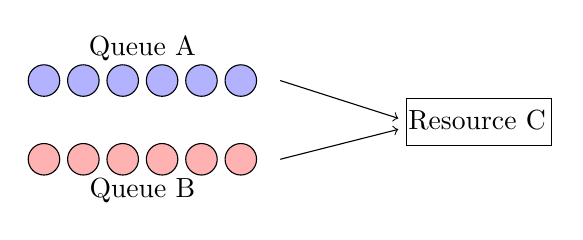
\begin{tikzpicture}
  % Queue A items (circles)
  \foreach \i in {0,...,5}
    \draw[fill=blue!30] (0.5cm + \i*0.5cm, 0) circle [radius=0.2cm];
  \node at (1.75cm, 0.4cm) {Queue A};

  % Queue B items (circles)
  \foreach \i in {0,...,5}
    \draw[fill=red!30] (0.5cm + \i*0.5cm, -1cm) circle [radius=0.2cm];
  \node at (1.75cm, -1.4cm) {Queue B};

  % Shared Resource C
  % \draw (6cm, -0.5cm) rectangle (4cm,3cm);
  \draw[draw=black] (5.1cm,-.83cm) rectangle ++(1.85,0.6);
  \node at (6cm, -0.5cm) {Resource C};

  % Arrows
  \draw[->] (3.5cm, 0cm) -- (5cm, -0.48cm);
  \draw[->] (3.5cm, -1.0cm) -- (5cm, -0.62cm);
\end{tikzpicture}
\caption{Diagram of Concurrency}
\end{figure}

\begin{figure}[ht]
\centering
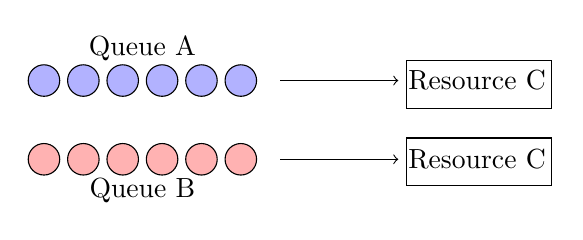
\begin{tikzpicture}
  % Queue A items (circles)
  \foreach \i in {0,...,5}
    \draw[fill=blue!30] (0.5cm + \i*0.5cm, 0) circle [radius=0.2cm];
  \node at (1.75cm, 0.4cm) {Queue A};

  % Queue B items (circles)
  \foreach \i in {0,...,5}
    \draw[fill=red!30] (0.5cm + \i*0.5cm, -1cm) circle [radius=0.2cm];
  \node at (1.75cm, -1.4cm) {Queue B};

  % Shared Resource C
  % \draw (6cm, -0.5cm) rectangle (4cm,3cm);
  \draw[draw=black] (5.1cm,-.35cm) rectangle ++(1.85,0.6);
  \node at (6cm, -0cm) {Resource C};
  \draw[draw=black] (5.1cm,-1.33cm) rectangle ++(1.85,0.6);
  \node at (6cm, -1.0cm) {Resource C};

  % Arrows
  \draw[->] (3.5cm, 0cm) -- (5cm, 0cm);
  \draw[->] (3.5cm, -1.0cm) -- (5cm, -1.0cm);
\end{tikzpicture}
\caption{Diagram of Parallelism}
\end{figure}

\subsection{Threads}
Java supports concurrent programming through its Thread API, but what is a thread? In essence, a \emph{thread} is a single lightweight process that executes a task, or a sequential set of tasks. 

\myexample{Multiple threads may access shared data at the same time, which is convenient. The problem is the fact that threads can \emph{context switch} at arbitrary points, which may include during an \emph{atomic operation}. Atomic operations are operations that must be executed in their entirety, without interruption. For example, suppose that we have a variable \ttt{counter} that we want to increment. We might write the following code:}

\begin{lstlisting}[language=MyJava]
import java.lang.Thread;
import java.lang.Runnable;

class RaceConditionExample {

  private static int counter = 0;

  public static void main(String[] args) {
    Thread t1 = new Thread(new Incrementer());
    Thread t2 = new Thread(new Incrementer());

    t1.start();
    t2.start();

    try {
      t1.join();
      t2.join();
    } catch (InterruptedException ex) { 
      ex.printStackTrace(); 
    }
    
    System.out.println(counter);
  }

  private static class Incrementer implements Runnable {

    @Override
    public void run() {
      for (int i = 0; i < 1_000_000; i++) { counter += 1; }
    }
  }
}
\end{lstlisting}

Upon running the program, we might expect the output to be \ttt{2_000_000}, but this is not the case. The output is nondeterministic, meaning that it is not guaranteed to be the same every time we run the program. This is because the \ttt{counter += 1} operation is not atomic. That is, the following sequence of events can occur:

\begin{enumerate}
  \item Thread $t_1$ reads the value of \ttt{counter} as \ttt{0}.
  \item Thread $t_2$ reads the value of \ttt{counter} as \ttt{0}.
  \item Thread $t_1$ increments the value of \ttt{counter} to \ttt{1}.
  \item Thread $t_2$ increments the value of \ttt{counter} to \ttt{1}.
  \item Thread $t_1$ writes the value of \ttt{counter} as \ttt{1}.
  \item Thread $t_2$ writes the value of \ttt{counter} as \ttt{1}.
\end{enumerate}

Thus, we need a way of synchronizing access to the \ttt{counter} variable. We will discuss this, alongside a more-detailed example, in the next section.

\subsubsection*{Synchronization}

\myexample{Let's suppose that we're writing a Java class to represent a bank account, which allows users to withdraw and deposit money. Further suppose that we have multiple threads that access the same bank account at once, eah depositing then immediately withdrawing five hundred dollars.}

\begin{lstlisting}[language=MyJava]
class BankAccount {

  private int amt;

  BankAccount(int amt) { 
    this.amt = amt; 
  }

  void deposit(int more) { 
    this.amt += more; 
  }

  void withdraw(int less) {
    if (amt >= less) { 
      this.amt -= less; 
    } else { 
      System.err.printf("withdraw: insufficient funds %d\n", less); 
    }
  }

  int getAmount() { 
    return this.amt; 
  }
}
\end{lstlisting}

Let's design a \ttt{TransactionThread} class, that implements \ttt{Runnable}, which executes one thousand ``transactions,'' i.e., a deposit of \$500, then a withdrawal of \$500.\footnote{It is an implementer's choice to either extend the \ttt{Thread} class or implement the \ttt{Runnable} interface. We choose the latter because Java allows us to implement multiple interfaces, but we can only extend one parent class. This does, however, mean that any time we want to instantiate a thread, we must also instantiate a separate instance of the \ttt{Runnable} subtype.} At the end, assuming everything works as expected, we should net zero dollars in the account.

\begin{lstlisting}[language=MyJava]
import java.lang.Runnable;

class TransactionThread implements Runnable {

  private BankAccount acc;

  TransactionThread(BankAccount acc) { 
    this.acc = acc; 
  }

  @Override
  public void run() {
    for (int i = 0; i < 1000; i++) {
      this.acc.deposit(500);
      this.acc.withdraw(500);
    }
  }
}
\end{lstlisting}

\begin{lstlisting}[language=MyJava]
import java.lang.Thread;

class BankAccountRunner {

  static void runTransactionThreads() {
    BankAccount acc = new BankAccount(0);
    Thread t1 = new Thread(new TransactionThread(acc));
    Thread t2 = new Thread(new TransactionThread(acc));
    Thread t3 = new Thread(new TransactionThread(acc));

    t1.start();
    t2.start();
    t3.start();

    // Wait on the threads to finish, then print the result.
    try {
      t1.join();
      t2.join();
      t3.join();
    } catch (InterruptedException ex) { 
      ex.printStackTrace(); 
    }

    System.out.printf("%d\n", acc.getAmount());
  }

  public static void main(String[] args) {
    runTransactionThreads();
  }
}
\end{lstlisting}

Running the program may produce the following output:

\begin{verbnobox}[\small]
withdraw: insufficient funds
withdraw: insufficient funds
0
\end{verbnobox}

It seems that we have an unpredictable problem: rerunning the program produces different results each time, but the error stems from the fact that our accesses to the bank account are not \emph{synchronized}. To understand why, let's expand out the code for performing a withdraw.

\begin{verbnobox}[\small]
void withdraw(int less) {
  int currAmt = this.amt;
  if (currAmt >= less) {
    int newAmt = currAmt - less;
    this.amt = newAmt;
  } else {
    // ... print not shown.
  }
}
\end{verbnobox}

\begin{sloppypar}{Recall how threads work---a thread $t_1$ might reach the third line of this method, and store some value in \ttt{newAmt}. At this point, suppose another thread $t_2$ makes a deposit of \$500. Finally, $t_1$ updates \ttt{newAmt} to zero, because \ttt{currAmt - less} must be zero, so we effectively nullify the deposit action by our second thread! As we showed with the previous example, this is a data race for the \ttt{amt} instance variable. To fix the problem, we want to ensure that our \ttt{withdraw} and \ttt{deposit} methods are synchronized, which we can do via marking the methods as \ttt{synchronized}. Synchronization of a method solves the problem of atomicity, i.e., a synchronized method can only be accessed by a single thread at any time. Let's mark our methods then rerun the code to check the result, which should never display an error. Even though the calls to \ttt{deposit} and \ttt{withdraw} might not be inside a synchronized environment, we end up netting zero in the account, because three successive calls to \ttt{deposit} must be followed, at some point, by three calls to \ttt{withdraw}, which our synchronization action guarantees.}
\end{sloppypar}

\myexample{Let's design a \ttt{transfer} method as part of the \ttt{BankAccount} class, which receives another \ttt{BankAccount} $b_2$ and an amount $n$ as an instance variable. We will transfer $n$ dollars from \ttt{this} bank into $b_2$, which resolves to a call to \ttt{withdraw} on \ttt{this} and a call to \ttt{deposit} on $b_2$.}

\begin{lstlisting}[language=MyJava]
import static Assertions.assertAll;
import static Assertions.assertEquals;

class BankAccountTester {

  @Test
  void testTransfer() {
    BankAccount b1 = new BankAccount(0);
    BankAccount b2 = new BankAccount(100);
    assertAll(
      () -> b2.transfer(b1, 30),
      () -> assertEquals(30, b1.getAmount()),
      () -> assertEquals(70, b2.getAmount()));
  }
}
\end{lstlisting}

\begin{lstlisting}[language=MyJava]
class BankAccount {

  private int amt;

  BankAccount(int amt) { 
    this.amt = amt; 
  }

  /**
   * Transfers money from one account to another.
   * @param b2 - other bank account to deposit money into.
   * @param amt - the amount to withdraw from this account.
   */
  void transfer(BankAccount b2, int amt) {
    this.withdraw(amt);
    b2.deposit(amt);
  }

  // deposit and withdraw not shown.
}
\end{lstlisting}

This code has the problem of not being synchronized; if multiple threads call \ttt{transfer} on the same bank account, we run into the same problem as before. To fix this, we may think that we need to synchronize \ttt{transfer}, but this is not the case, because a method that is synchronized means that only one thread can enter the method, but we need to synchronize the bank objects themselves from access and mutation. We can do so by synchronizing on the bank objects themselves, which we can do by using the \ttt{synchronized} keyword on a block of code. First, we synchronize on \ttt{this} (the bank account that we are withdrawing from), followed by a synchronization on \ttt{b2} (the bank account that we are depositing into). This ensures that only one thread can access both bank accounts concurrently.

Let's now create another class that implements \ttt{Runnable} to manage multiple transfers between bank accounts. Each thread will deposit \$500 into its first bank $b_1$, then transfer \$500 from $b_1$ to $b_2$, followed by a withdrawal of \$500 from $b_2$ to ensure that both accounts net zero dollars. Our tester will create two threads: one that transfers from $b_1$ to $b_2$, and another that transfers from $b_2$ to $b_1$.

\begin{lstlisting}[language=MyJava]
import java.lang.Runnable;

class TransferThread implements Runnable {

  private final BankAccount B1;
  private final BankAccount B2;

  TransferThread(BankAccount b1, BankAccount b2) {
    this.B1 = b1;
    this.B2 = b2;
  }

  @Override
  public void run() {
    for (int i = 0; i < 1000; i++) { 
      this.B1.transfer(this.B2, 500); 
    }
  }
}
\end{lstlisting}

\begin{lstlisting}[language=MyJava]
import java.lang.Thread;

class BankAccountRunner {

  static void runTransferThreads() {
    BankAccount b1 = new BankAccount(0);
    BankAccount b2 = new BankAccount(0);
    Thread t1 = new Thread(new TransferThread(b1, b2));
    Thread t2 = new Thread(new TransferThread(b2, b1));

    t1.start();
    t2.start();

    try {
      t1.join();
      t2.join();
    } catch (InterruptedException ex) { 
      ex.printStackTrace(); 
    }
  }

  public static void main(String[] args) {
    runTransferThreads();
  }
}
\end{lstlisting}

\begin{lstlisting}[language=MyJava]
class BankAccount {

  private int amt;

  BankAccount(int amt) { 
    this.amt = amt; 
  }

  /**
   * Transfers money from one account to another.
   * @param b2 - other bank account to deposit money into.
   * @param amt - the amount to withdraw from this account.
   */
  void transfer(BankAccount b2, int amt) {
    synchronized (this) {
      synchronized (b2) {
        this.withdraw(amt);
        b2.deposit(amt);
      }
    }
  }

  // deposit and withdraw not shown.
}
\end{lstlisting}

Upon running this program it is very likely to encounter an unexpected problem: an infinite ``loop,'' so to speak. This occurs because we have a \emph{deadlock}\index{deadlock}, which happens when two more more threads are waiting on each other to release a lock. In our case, thread $t_1$ synchronizes on itself and acquires the lock. Then, suppose we context switch into $t_2$ and it synchronizes on itself. At this point $t_1$ is waiting for the lock by $t_2$, and $t_2$ is waiting on $t_1$'s lock. There are several possible solutions to this problem, where one is to use a Java-defined \ttt{Lock} object. As we will discuss in the subsequent example, a reentrant lock allows a thread to acquire the lock multiple times, which is useful in the event that a thread needs to call a synchronized method from within a synchronized block. In particular, we will lock \ttt{transfer}, \ttt{deposit}, and \ttt{withdraw} using the same static lock. We will also use a \ttt{try/finally} block to ensure that the lock is released, even if an exception is thrown.

\begin{lstlisting}[language=MyJava]
class BankAccount {

  private int amt;

  private static Lock lock = new ReentrantLock();

  BankAccount(int amt) {
    this.amt = amt;
  }

  /**
   * Transfers money from one account to another.
   * @param b2 - other bank account to deposit money into.
   * @param amt - the amount to withdraw from this account.
   */
  void transfer(BankAccount b2, int amt) {
    BankAccount.lock.lock();
    try {
      this.withdraw(amt);
      b2.deposit(amt);
    } finally {
      BankAccount.lock.unlock();
    }
  }

  void deposit(int more) {
    BankAccount.lock.lock();
    try { this.amt += more; } 
    finally {  BankAccount.lock.unlock(); }
  }

  void withdraw(int less) {
    BankAccount.lock.lock();
    try {
      if (amt >= less) { this.amt -= less; }
      else { System.err.printf("withdraw: insufficient funds\n"); }
    } finally {
      BankAccount.lock.unlock();
    }
  }
}
\end{lstlisting}

\myexample{A \emph{thread-safe data structure} is one that supports reentrancy, i.e., multiple threads working over it at the same time. Java's \ttt{ArrayList} class is not thread-safe, so we will implement our own thread-safe array list using locks. The idea is to wrap all pieces of the code that multiple threads may access with a lock. Recalling our \ttt{MiniArrayList} class from Chapter~\ref{chapter:classes}, we see that \ttt{add}, \ttt{remove}, \ttt{insert}, \ttt{get}, and \ttt{size} all either access or modify the state of the list, which could conflict with another thread and cause a dangerous race condition. Thus we will surround the code within a lock. Note that some methods do not, themselves, need to be synchronized, e.g., \ttt{shiftLeft}/\ttt{shiftRight}/\ttt{resize}, because they are only ever called from within a synchronized context. Should we wrap those methods in the same lock, then the thread who owns the lock would be unable to call those methods, causing a deadlock.\footnote{As we showed with the bank account example, Java's \ttt{ReentrantLock} class is reentrant, meaning that a thread can safely acquire the lock multiple times. So, this problem is not necessarily an issue, but we will still avoid it for the sake of clarity and adaptability to other languages that may not have reentrant locks.} Moreover, because the \ttt{remove} method calls \ttt{get}, acquiring the lock immediately in \ttt{remove} is a bad idea. So, we acquire the lock in \ttt{get}, then release it, then acquire it again in \ttt{remove}. Certain methods, e.g., \ttt{size} and \ttt{get}, need to be updated to account for releasing the lock before the return statement; in these cases we store the result in a (local) temporary variable, release the lock, then return. In the code segment, we omit the comments for the sake of brevity. In all cases, we use \ttt{try/finally} blocks to ensure that, even in the case of exceptions, the lock is released, which is especially important with data structural methods.}

\begin{lstlisting}[language=MyJava]
import java.util.concurrent.locks.Lock;
import java.util.concurrent.locks.ReentrantLock;

class ThreadSafeArrayList<T> {
  // ... other instance variables not shown.
  private Lock lock;

  ThreadSafeArrayList(int capacity) {
    this.size = 0;
    this.capacity = capacity;
    this.elements = (T[]) new Object[capacity];
    this.lock = new ReentrantLock();
  }

  void add(T element) {
    this.lock.lock();
    if (this.size == this.capacity) { this.resize(); }
    this.elements[this.size] = element;
    this.size++;
    this.lock.unlock();
  }

  void insert(T e, int idx) {
    this.lock.lock();
    try {
      if (this.size == capacity) { this.resize(); }
      this.shiftRight(idx);
      this.elements[idx] = e;
    } finally { this.lock.unlock(); }
  }

  T remove(int idx) {
    this.lock.lock();
    try {
      T e = this.get(idx);
      this.shiftLeft(idx);
      this.size--;
    } finally { this.lock.unlock(); }
    return e;
  }

  T get(int index) {
    this.lock.lock();
    try { T e = this.elements[index]; }
    finally { this.lock.unlock(); }
    return e;
  }

  int size() {
    this.lock.lock();
    try { int sz = this.size; }
    finally { this.lock.unlock(); }
    return sz;
  }
}
\end{lstlisting}

Java, in fact, does have a data structure in the Collections API that supports multithreading and is therefore thread-safe: the \ttt{Vector} class serves this purpose. Though, should we not want to use \ttt{Vector}, since some Java programmers consider it ``deprecated,'' we can invoke the static \ttt{synchronizedList} method on \ttt{Collections} to return a synchronized/thread-safe version of the input list. There are also other data structures in the Collections API that are thread-safe, such as \ttt{ConcurrentHashMap} and \ttt{ConcurrentLinkedQueue}, as well as methods to convert a non-thread-safe data structure into one that is thread-safe, e.g., \ttt{synchronizedMap} and \ttt{synchronizedSet}.

\myexample{In the event that we want to block concurrent access to a variable, we need to enforce a few more precautions than simply marking methods that access the variable as \ttt{synchronized}. Moreover, should we want to not deal with locks but still require atomic operations over access to an integer, we can use, for example, \ttt{AtomicInteger}. Let's revisit the \ttt{counter} example from earlier, but this time we will use an \ttt{AtomicInteger} to ensure that the increment operation is atomic.}

\begin{lstlisting}[language=MyJava]
import java.util.concurrent.atomic.AtomicInteger;
import java.lang.Thread;
import java.lang.Runnable;

class AtomicIntegerExample {

  private static AtomicInteger counter = new AtomicInteger(0);

  public static void main(String[] args) {
    Thread t1 = new Thread(new Incrementer());
    Thread t2 = new Thread(new Incrementer());

    t1.start();
    t2.start();

    try {
      t1.join();
      t2.join();
    } catch (InterruptedException ex) { 
      ex.printStackTrace(); 
    }

    System.out.println(counter);
  }

  private static class Incrementer implements Runnable {

    @Override
    void run() {
      for (int i = 0; i < 1_000_000; i++) { 
        inc(); 
      }
    }

    static synchronized void inc() {
      counter.incrementAndGet();
    }
  }
}
\end{lstlisting}

% \myexample In the event that we only want to block concurrent access to a variable, we can wrap the operation that we want to be atomic inside a \ttt{synchronized} block. A method that is synchronized can only be accessed by one thread at a time, and all other threads that attempt to access the method will block until the lock is released. We can also synchronize on a specific object, which is useful when we want to synchronize on a variable that is not a method. In the following example, we synchronize on the \ttt{counter} variable, which is not a method. We can also synchronize on the class itself, which is useful when we want to synchronize on a static method.


\subsubsection*{Condition Variables}

\myexample{Imagine that we are writing a multithreaded program, where thread $t_1$ is a ``consumer,'' and there are multiple ``producer'' threads $t_2, \ldots, t_n$. The producer threads add data to a list, and the consumer polls them when available. We want to ensure that the consumer only polls the list when it is non-empty. So, one might think to write the following code for the consumer:}

\begin{lstlisting}[language=MyJava]
import java.lang.Runnable;
import java.util.Vector;

class Consumer<T> implements Runnable {

  private final Vector<T> LIST;

  Consumer(Vector<T> ls) { this.LIST = ls; }

  @Override
  public void run() {
    while (true) {
      while (this.LIST.isEmpty()) { /* Do nothing. */ }
      T e = this.LIST.remove(0);
      System.out.printf("Consumed: %s\n", e.toString());
    }
  }
}
\end{lstlisting}

The consumer thread will ``busy-wait'' until the list is non-empty. A busy-wait loop is not recommended because the thread has to continuously check the list to determine if an element exists, which is wasteful. Plus, there's the added problem that this code is not thread-safe; by not acquiring a lock, we run into the potential of a race condition where one thread polls the queue and another is about to poll the queue. Even though our queue definition \emph{is} thread-safe, this does not solve the problem of a thread trying to remove an element that does not exist outside the fact. The solution is to use a \emph{condition variable}, which serves as a signal between threads. While the list is empty, our consumer thread awaits on the condition variable, thereby putting it to sleep. Then, the producer thread(s) will issue a signal to the condition variable when inserting data into the list. Condition variables are always associated with a lock, so we need to define one in our main program and pass it around to both the producer(s) and consumer. 

When the consumer acquires the lock, it checks if the list is empty. If so, it awaits on the condition variable, which releases the held lock and puts the thread to sleep. When the producer acquires the lock, it adds an element to the list, then issues a signal to the condition variable, which wakes up the consumer thread. The signal causes the consumer to reacquire the lock, check if the list is empty, and, if not, remove (and process) the head element from the list, followed by releasing the lock.

For the sake of our example, suppose that a producer adds data to the list using a random number generator.\footnote{The \ttt{Random} class is thread-safe.} That is, we generate a random number, determine if it is within a specific range and, if so, add data to the list. This then means that the producer thread signals on the condition variable, awaking the consumer.

\begin{lstlisting}[language=MyJava]
import java.util.concurrent.locks.Condition;
import java.util.concurrent.locks.Lock;
import java.util.Random;
import java.util.Vector;

class Producer implements Runnable {

  private static final Random RAND = new Random();

  private final Vector<Integer> LIST;
  private final Lock LOCK;
  private final Condition COND_VAR;

  Producer(Vector<Integer> ls, Lock lock, Condition condVar) {
    this.LIST = ls;
    this.LOCK = lock;
    this.COND_VAR = condVar;
  }

  @Override
  public void run() {
    while (true) {
      this.LOCK.lock();
      int n = this.RAND.nextInt(100);
      if (n < 10) {
        this.LIST.add(n);
        this.COND_VAR.signal();
      }
      this.LOCK.unlock();
    }
  }
}
\end{lstlisting}

Further note that awaiting on a condition variable may throw an \ttt{InterruptedException}, meaning we must surround the call with a \ttt{try/catch} block.\footnote{Should we not want to do this, we can instead invoke the \ttt{awaitUninterruptibly} method.} An important fact to also consider is that, if a thread that issues a signal on a condition variable does not own the respective lock, Java will throw an \ttt{IllegalMonitorStateException}.

\begin{lstlisting}[language=MyJava]
import java.util.concurrent.locks.Condition;
import java.util.concurrent.locks.Lock;
import java.util.Random;
import java.util.Vector;
import java.lang.Thread;

class ConditionVariableExample {

  private static final Lock LOCK = new ReentrantLock();
  private static final Condition COND_VAR = LOCK.newCondition();
  private static final Vector<Integer> LIST = new Vector<>();

  public static void main(String[] args) {
    Thread t1 = new Thread(new Consumer<>(LIST, LOCK, COND_VAR));
    Thread t2 = new Thread(new Producer<>(LIST, LOCK, COND_VAR));
    Thread t3 = new Thread(new Producer<>(LIST, LOCK, COND_VAR));

    t1.start();
    t2.start();
    t3.start();
  }
}
\end{lstlisting}

If we fix our input seed to \ttt{212}, the output is deterministically as follows:

\begin{verbnobox}[\small]
Consumed: 1
Consumed: 6
Consumed: 1
Consumed: 7
Consumed: 7
Consumed: 8
Consumed: 1
Consumed: 4
Consumed: 5
\end{verbnobox}

\subsection{Networking \& Sockets}

Computers that communicate with one another is not a revolutionary idea, but being able to write programs that act as \emph{clients} and \emph{servers} is certainly cool. A server is a program that listens for incoming connections over a network and processes them accordingly. Clients connect to servers to do different things, e.g., receive information from a server, talk to other connected clients, and so on. In this section we will demonstrate the Java networking/socket API and how to write a few programs that incorporate a server.

\myexample{The simplest kind of server is one that receives an incoming connection and outputs/relays some data to the client, then closes said connection. Our first example using a server will accept a client, then tell it the current server clock date and time, then close the connection. Servers operate on \emph{ports} over a connection, which, simply put, are virtual places where connections occur. Our server will be hosted on port $8080$: a common default port. So, we instantiate an object of type \ttt{ServerSocket} to listen on $8080$, and set up an infinite loop to forever listen for connections. Upon receiving one, we accept the client as a \ttt{Socket}, we instantiate a data stream to print information out to the client. One important detail to note is that we need to designate the \ttt{PrintWriter} output stream to ``autoflush'' its data. In essence, this means that as soon as the client reads data from the server, it gets emitted to their standard output stream. Note that we do not need to declare a reader stream from the client, since our server does not receive data.}

The server \emph{blocks} until it receives a connection, similar to how many of the input reader classes, e.g., \ttt{Scanner}, \ttt{BufferedReader}, wait until data is sent to the input stream to continue execution. A blocking server that is implemented in this fashion, as we have done, can only serve one client at a time, since it has to accept the client, set up the output stream, print the data, then close the connection before being able to accept another.

\begin{lstlisting}[language=MyJava]
import java.io.IOException;
import java.io.OutputStreamWriter;
import java.io.PrintWriter;
import java.net.ServerSocket;
import java.net.Socket;

class TimeEchoServer {

  private static final int PORT = 8080;

  public static void main(String[] args) {
    try (ServerSocket ss = new ServerSocket(PORT)) {
      System.out.printf("Server listening on port %d...\n", PORT);
      // Continuously listen for clients.
      while (true) {
        // Accept the incoming client, block until we receive one.
        Socket client = ss.accept();
        System.out.printf("Client connected: %s\n", 
                          client.getInetAddress().toString());
        PrintWriter pw = new PrintWriter(
                          new OutputStreamWriter(
                            client.getOutputStream()), 
                            true);
        // Echo the server time to the client.
        pw.println("The server time is " + java.time.LocalDateTime.now());
        // Echo client disconnection, then close.
        System.out.printf("Client disconnected: %s\n", 
                          client.getInetAddress().toString());
        client.close();
      }
    } catch (IOException ex) { 
      ex.printStackTrace(); 
    }
  }
}
\end{lstlisting}

To connect to this server, we can use the Unix \ttt{nc} ``netcat'' command to connect to \ttt{localhost}, e.g., \ttt{nc localhost 8080}, while the server is running.

\myexample{Let's write a server that, upon receiving a connection, allows the client to type a number. This number is then translated by the server into an index, grabbing them the $n^{\text{th}}$ most populous country. So, our server first must read in a list of countries from most populous to least. From there we establish the same server connection, only this time we must use both the input and output streams of the client, so we can read the number that they enter, as well as output the corresponding country.} 

\begin{lstlisting}[language=MyJava]
import java.io.IOException;
import java.io.InputStreamReader;
import java.io.OutputStreamWriter;
import java.io.PrintWriter;
import java.net.ServerSocket;
import java.net.Socket;
import java.util.List;

class CountryPopulationRankServer {

  private final int PORT;
  private final List<String> COUNTRIES;

  CountryPopulationRankServer(int port) {
    this.PORT = port;
    this.COUNTRIES = new ArrayList<>();

    // Read in the words from the text file.
    try (BufferedReader br = new BufferedReader(new FileReader("clist.txt"))) {
      String line = null;
      while ((line = br.readLine()) != null) { 
        this.COUNTRIES.add(line); 
      }
    } catch (IOException ex) { 
      ex.printStackTrace(); 
    }
  }

  void start() {
    // Set up the thread pool.
    try (ServerSocket ss = new ServerSocket(this.PORT)) {
      while (true) {
        Socket s = ss.accept();
        BufferedReader br = new BufferedReader(
                              new InputStreamReader(s.getInputStream()));
        // Read in the country from the user.
        String line = br.readLine();
        int country = Integer.parseInt(line) - 1;
        PrintWriter pw = new PrintWriter(socket.getOutputStream(), true);
        // Output the nth most populous country.
        pw.printf("%d country: %s\n", country + 1, 
                  this.COUNTRIES.get(country));
        socket.close();
      }
    } catch (IOException ex) { 
      ex.printStackTrace(); 
    }
  }

  public static void main(String[] args) {
    new CountryPopulationRankServer(8080).start();
  }
}
\end{lstlisting}

\myexample{Let's use what we have learned to write a \emph{multithreaded} chat server. That is, we will write a program that acts as server for a chat room. Clients can connect to the server and send messages to each other. The server will be multithreaded so that it can simultaneously serve clients. First, we need to decide on a protocol for communication between the server and the clients. For this example, to minimize the number of features necessary to convey the important ideas, we will only allow the user to log into the ``room,'' type messages to all users in the room, or to disconnect via the \ttt{\textbackslash{quit}} command. The server houses a \emph{thread pool} that spins up a thread to communicate with a connected client. Fortunately for us, because we are in Java, we have access to synchronized data structures such as \ttt{Vector}. Therefore, we do not need to manually insert locks into a data structure for storing those connected clients. After a server receives a client, as we stated, we dedicate a thread to that user, then resume listening. We will also have a server thread that actively listens for messages that are then relayed to every other user. The notion of the server having a thread to listen for messages is known as a \emph{task-handler}, whose tasks are queued away in a synchronized \ttt{LinkedBlockingQueue} data structure. When reading a command from the user, we enqueue it into the server's queue of tasks, which blocks until a task is available. The task-handler then dequeues the task and broadcasts it to all users. It will be up to the client to determine whether or not they are the intended recipient.}\footnote{From a security standpoint, broadcasting a message in this fashion is incredibly insecure, since a client can simply decide if it is the intended recipient no matter if the message is not intended for them.}

\begin{lstlisting}[language=MyJava]
import java.lang.Runnable;

class Server {
  // ... other data not shown.

  private static class TaskHandler implements Runnable {

    private final Server SERVER;

    TaskHandler(Server server) { 
      this.SERVER = server; 
    }

    @Override
    public void run() {
      while (this.SERVER.running) {
        try {
          Task task = this.SERVER.TASKS.take();
          this.SERVER.CLIENTS.forEach(c -> c.send(task));
        } catch (InterruptedException e) { 
          e.printStackTrace(); 
        }
      }
    }
  }
}
\end{lstlisting}

\begin{lstlisting}[language=MyJava]
import java.util.concurrent.BlockingQueue;
import java.util.concurrent.LinkedBlockingQueue;
import java.util.concurrent.ExecutorService;
import java.util.Vector;
import java.net.ServerSocket;
import java.net.Socket;
import java.io.IOException;

class Server {

  private final ExecutorService THREAD_POOL;
  private final Vector <Client> CLIENTS;
  private final BlockingQueue <Task> TASKS;
  private final int PORT;
  private boolean running;

  Server(int port) {
    this.running = true;
    this.PORT = port;
    this.THREAD_POOL = Executors.newCachedThreadPool();
    this.CLIENTS = new Vector<>();
    this.TASKS = new LinkedBlockingQueue<>();
    this.THREAD_POOL.execute(new TaskHandler(this));
  }

  void start() {
    try {
      ServerSocket server = new ServerSocket(this.PORT);
      System.out.printf("Server connected on port %d...\n", this.PORT);
      while (this.running) {
        Socket client = server.accept();
        System.out.printf("Client %s connected!\n", 
                          client.getInetAddress());
        Client c = new Client(client, this);
        this.CLIENTS.add(c);
        this.THREAD_POOL.execute(c);
      }
    } catch (IOException e) { e.printStackTrace(); }
  }

  void addTask(Task t) {
    if (t != null) { this.TASKS.add(t); }
  }

  public static void main(String[] args) { new Server(8080).start(); }
}
\end{lstlisting}

Clients contain an output and input stream, which are used to send and receive messages to and from the server, as we saw with the country population ranking server. The client thread is responsible for reading messages from the server and printing them to the user's console, as well as receiving messages from the clients' standard input stream, and feeding those lines to the server. We will also designate that a client has a user identifier and stores a flag indicating whether or not the client is "logged in", which simply represents if they can receive broadcast messages. By default, the user identifier will be the IP address of the connected socket, which is replaceable/alterable via the \ttt{"login"} command. Moreover, in case a client disconnects from the server, we utilize the \ttt{connected} flag to prevent the thread from reusing the now-closed input stream. We will disable this flag once we implement the functionality for handling quit commands.

\begin{lstlisting}[language=MyJava]
import java.io.IOException;
import java.io.BufferedReader;
import java.io.PrintWriter;
import java.lang.Runnable;
import java.net.ServerSocket;
import java.net.Socket;

class Client implements Runnable {

  private final Socket SOCKET;
  private final Server SERVER;
  private final BufferedReader IN;
  private final PrintWriter OUT;

  private boolean loggedIn;
  private boolean connected;
  private String userId;

  Client(Socket socket) {
    this.SOCKET = socket;
    this.SERVER = server;
    this.IN = new BufferedReader(
                new InputStreamReader(socket.getInputStream()));
    this.OUT = new PrintWriter(socket.getOutputStream(), true);
    this.loggedIn = false;
    this.connected = true;
    this.userId = socket.getInetAddress().toString();
  }

  @Override
  public void run() {
    try {
      String line;
      while (this.connected && (line = this.IN.readLine()) != null) { 
        this.SERVER.addTask(parseCmd(line)); 
      }
    } catch (IOException e) { e.printStackTrace(); }
  }
}
\end{lstlisting}

We now need to write the \ttt{parseCmd} message, which receives an unparsed string from the client and returns a \ttt{Task} object, which we will design momentarily. Commands, in our system, will be prefixed via a forward slash \ttt{/}, followed by the arguments thereof. As an example, \ttt{/login joshua} will set the user's identifier to \ttt{joshua}. We will also allow the user to send messages to all other users via the \ttt{/send} command, which is followed by the message broadcast. Finally, the \ttt{/quit} command disconnects the user from the server.

\begin{lstlisting}[language=MyJava]
class Client {
  // ... other information not shown.

  Task parseCmd(String line) {
    String cmd = line.substring(0, line.indexOf(' '));
    String msg = line.substring(line.indexOf(' ') + 1);
    switch (cmd) {
      case "/login" -> { return this.handleLoginCmd(msg); }
      case "/send"  -> { return this.handleSendCmd(msg); }
      case "/quit"  -> { return this.handleQuitCmd(); }
      default -> throw new IllegalArgumentException("bad cmd " + cmd);
    }
  }
}
\end{lstlisting}

Our tasks will consist of a hierarchy of objects. Namely, a \ttt{Task} contains an enumeration of its type, as well as the raw data. A \ttt{SenderTask} is a task that contains a sender information, which stores an instance variable denoting the \ttt{Client} who the message originated from. Finally, a \ttt{BroadcastTask} is a task that contains a message to be broadcast to all users, which is itself a subclass of \ttt{SenderTask}. Tasks are operations that must be sent to the server and handled by one of its threads. Certain commands may remain local to the server due to their simplicity, e.g., \ttt{"/login"} and \ttt{"/quit"} do not need to be relayed to other users (and therefore are not wrapped as \ttt{Task} instances). 

\begin{lstlisting}[language=MyJava]
enum TaskType { BROADCAST }
\end{lstlisting}

\begin{lstlisting}[language=MyJava]
abstract class Task {

  private final TaskType TYPE;
  private final String RESPONSE;

  Task(TaskType type, String response) {
    this.TYPE = type;
    this.RESPONSE = response;
  }

  TaskType getType() { return this.TYPE; }

  String getResponse() { return this.RESPONSE; }
}
\end{lstlisting}

\begin{lstlisting}[language=MyJava]
abstract class SenderTask extends Task {

  private final Client SENDER;

  SenderTask(TaskType type, String response, Client sender) {
    super(type, response);
    this.SENDER = sender;
  }

  Client getSender() { return this.SENDER; }
}
\end{lstlisting}

\begin{lstlisting}[language=MyJava]
class BroadcastTask extends SenderTask {

  BroadcastTask(Client sender, String response) {
    super(TaskType.BROADCAST, response, sender);
  }
}
\end{lstlisting}

We now must write the \ttt{Client}'s \ttt{send} method, which receives a \ttt{Task} from the server and interprets it accordingly. The only task that our server can send is \ttt{BROADCAST}, so we simply need to check whether the client is logged in and, if so, print the message to their output stream. At the same time, we can also take care of privatized parsing command methods. Only one of these three should return a non-\ttt{null} object. It is also a design decision to make \ttt{handleQuitCmd} and \ttt{handleLoginCmd} return \ttt{null} because they do not need to be broadcast to other users. We do so to ensure consistency among the methods.

\begin{lstlisting}[language=MyJava]
class Client {
  // ... other information not shown.

  void send(Task t) {
    switch (t) {
      case BroadcastTask tb -> {
        if (this.loggedIn) { 
          this.OUT.printf("%s: %s\n", tb.getSender(), tb.getResponse()); 
        }
      }
      default -> {
        throw new IllegalArgumentException("bad task "+t.getType());
      }
    }
  }

  private Task handleLoginCmd(String msg) {
    this.userId = msg;
    this.loggedIn = true;
    return null;
  }

  private Task handleSendCmd(String msg) {
    return new BroadcastTask(this, msg);
  }

  private Task handleQuitCmd() {
    this.loggedIn = false;
    try {
      this.SOCKET.close();
      this.IN.close();
      this.OUT.close();
    } 
    catch (IOException e) { e.printStackTrace(); }
    finally { return null; }
  }
}
\end{lstlisting}

Now we can run the server! Clients connect via the ``netcat'' command \ttt{nc}, which is a Unix utility for reading and writing to network connections. We can connect to the server, using multiple terminals, via \ttt{nc localhost 8080}. Below is a demo of the server running with three clients connected.